\cleardoublepage

\chapter{Introducción}
\label{makereference}

El objetivo de este proyecto es predecir la radiación solar en un plazo de treinta minutos. Para ello debemos hacer un estudio de los distintos algoritmos de predicción y de los parámetros meteorólogicos determinantes para obtener dicha predicción.

% Mirar descripción inicial TFG y Drive

\begin{figure}[htb]%t=top, b=bottom, h=here
	
	\begin{center}
		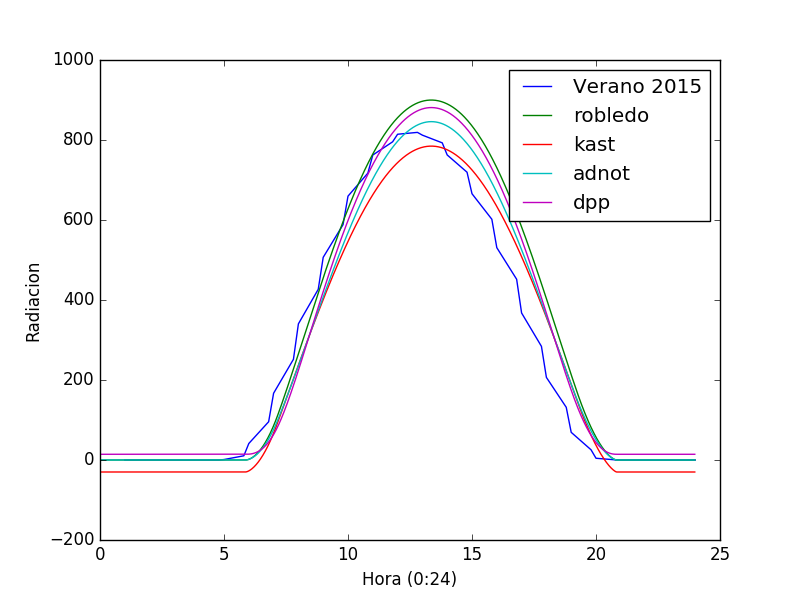
\includegraphics[height=2.5in]{figures/verano2015.png}
		\caption{Modelo verano 2015}
	\end{center}
    
    \label{figure1}
\end{figure}

% +--------------------------------------------------------------------+
% |To create cross-references to figures, tables and segments
% |of text, LaTeX provides the following commands:
% |   \label{marker}
% |   \ref{marker}
% |   \pageref{marker}
% | where {marker} is a unique identifier.
% |
% | In the line above, we use \label{figure1} to mark a location
% | we wish to refer to later.  LATEX replaces \ref by the number of
% | the chapter, section, subsection, figure, or table after which the
% | corresponding \label command was issued. \pageref prints the page
% | number of the page where the \label command occurred.
% |
% +--------------------------------------------------------------------+

\section{Motivación}
\label{makereference1.1}

En un principio decidimos hablar con nuestro futuro tutor de TFG, ya que habíamos tenido una muy buena experiencia como alumnos en su clase de Sistemas Operativos.
Nos propuso tres proyectos distintos: Control de temperatura en máquinas frigoríficas, control de accesos a grandes instituciones y este.

Nos decantamos por este proyecto debido a que nos pareció el más completo en cuanto a tecnologías a manejar y con el que más prodríamos aprender. Mucha implicación tanto hardware, como software. Queríamos hacer algo fuera de lo estudiado en la carrera.

Este proyecto nos ha supuesto aprender lenguajes que no conocíamos (python y matlab), reforzar otros (bash).

Además de todo esto, hace dos años cursamos una asignatura optativa llamada Minería de datos y el paradigma Big Data, la cual nos motivó bastante a la hora de elegir este proyecto. Nos gustaba mucho la idea de aprender algo de 'Machine Learning' y Python debido a que es un sector muy puntero y solicitado.

% Referenciar
In this paragraph, we want to refer to Fig.~\ref{figure1}
mentioned at the beginning of this chapter.  We also refer to the
Table~\ref{table1}.

\section{Breve descripción del sistema}
\label{makereference1.2}

Nuestro sistema cuenta con tres grandes módulos de trabajo: nodo, servidor, resultados.

El nodo es una Raspberry Pi a las que están conectados varios sensores que recogen muestras del entorno para su posterior tratamiento. Dichos datos serán enviados a un servidor alojado en la Facultad de Físicas donde se generará una predicción de la radiación solar.

El servidor, previamente entrenado con los datos meteorológicos que nos proporcionó nuestro tutor, predecirá la radiación a partir de los datos recibidos del nodo. 

Esa predicción será representada en ThinkSpeak mediante una gráfica junto a la radiación real.

In this section, we refer back to text mentioned in
Section~\ref{makereference1.1} on page~\pageref{makereference1.1}.

\section{Making a Citation}
\label{makereference1.3}

Here's an example of a citation to a single
work.~\cite{CT:Weiner:1999} It's also possible to make multiple
citations.~\cite{CT:Phillips:1985, ARP:Loy:1974}
